\documentclass{beamer}
\usepackage{gvv}
\usepackage[utf8]{inputenc}
\usepackage{enumitem}
\usetheme{Madrid}
\usecolortheme{default}
\usepackage{amsmath,amssymb,amsfonts,amsthm}
\usepackage{txfonts}
\usepackage{tikz}
\usepackage{graphicx}
\usepackage{minted}

\setbeamertemplate{page number in head/foot}[totalframenumber]
\renewcommand{\vec}[1]{\mathbf{#1}}
\title{1.8.22: Equidistant Points Problem}
\author{Aditya Mishra - ee25btech11005}
\date{September 9, 2025}

\begin{document}

\frame{\titlepage}
\begin{frame}{Question}
Find all points that are equidistant from
\[
\vec{A} = \myvec{-5 \\ 4}, \quad
\vec{B} = \myvec{-1 \\ 6}.
\]
How many such points exist?
\end{frame}

\begin{frame}{Given Information}
Points as column vectors:
\[
\vec{A} = \myvec{-5 \\ 4}, \quad
\vec{B} = \myvec{-1 \\ 6}.
\]
Desired point:
\[
\vec{O} = \myvec{x \\ y}.
\]
\end{frame}

\begin{frame}{Equidistant Condition}
Equidistant means:
\[
\norm{\vec{O} - \vec{A}} = \norm{\vec{O} - \vec{B}}.
\]
Squaring both sides:
\[
\norm{\vec{O} - \vec{A}}^2 = \norm{\vec{O} - \vec{B}}^2.
\]
Using vector dot product:
\[
(\vec{O} - \vec{A})^\top (\vec{O} - \vec{A}) = (\vec{O} - \vec{B})^\top (\vec{O} - \vec{B}).
\]
\end{frame}

\begin{frame}{Simplify the Equation}
Expand both sides:
\[
\vec{O}^\top \vec{O} - 2 \vec{A}^\top \vec{O} + \vec{A}^\top \vec{A} = \vec{O}^\top \vec{O} - 2 \vec{B}^\top \vec{O} + \vec{B}^\top \vec{B}.
\]
Simplify by cancelling \(\vec{O}^\top \vec{O}\):
\[
- 2 \vec{A}^\top \vec{O} + \vec{A}^\top \vec{A} = - 2 \vec{B}^\top \vec{O} + \vec{B}^\top \vec{B}.
\]
Rearranged:
\[
2 (\vec{B} - \vec{A})^\top \vec{O} = \vec{B}^\top \vec{B} - \vec{A}^\top \vec{A}.
\]
\end{frame}

\begin{frame}{Final Equation}
\[
(\vec{B} - \vec{A})^\top \vec{O} = \frac{\vec{B}^\top \vec{B} - \vec{A}^\top \vec{A}}{2}.
\]
Put terms explicitly:
\[
\myvec{4 & 2} \myvec{x \\ y} =
\frac{37 - 41}{2} = -2.
\]
That gives a line equation:
\[
4x + 2y = -2 \implies 2x + y = -1.
\]
\end{frame}

\begin{frame}{Number of Solutions}
The set of points equidistant from \(\vec{A}\) and \(\vec{B}\) lies on the line:
\[
2x + y = -1.
\]
There are infinitely many such points.
\end{frame}

\begin{frame}[fragile]{C Code: Equidistant Line Calculation}
\begin{minted}[fontsize=\footnotesize]{c}
#include <stdio.h>

void equidistant_line(double ax, double ay, double bx, double by,
double *res) {
    double a = bx - ax;
    double b = by - ay;
    double normA_sq = ax*ax + ay*ay;
    double normB_sq = bx*bx + by*by;
    double c = (normB_sq - normA_sq) / 2.0;

    res[0] = a;
    res[1] = b;
    res[2] = c;
}
\end{minted}
\end{frame}


\begin{frame}[fragile]{Python ctypes}
\begin{minted}[fontsize=\footnotesize]{python}
import ctypes

lib = ctypes.CDLL('./libequidistant.so')

lib.equidistant_line.argtypes = [
    ctypes.c_double, ctypes.c_double,
    ctypes.c_double, ctypes.c_double,
    ctypes.POINTER(ctypes.c_double),  # Output array for coeffs
]

lib.equidistant_line.restype = None

res = (ctypes.c_double * 3)()  # To hold a,b,c in ax + by = c

lib.equidistant_line(-5, 4, -1, 6, res)

print(f"Line: {res[0]} x + {res[1]} y = {res[2]}")
\end{minted}
\end{frame}
\begin{frame}[fragile]{Python Code: Plot Equidistant Line and Points}
\begin{minted}[fontsize=\footnotesize]{python}
import numpy as np
import matplotlib.pyplot as plt

A = np.array([-5, 4])
B = np.array([-1, 6])

a = B[0] - A[0]
b = B[1] - A[1]

c = (np.dot(B, B) - np.dot(A, A)) / 2
x = np.linspace(-10, 5, 400)
y = (c - a * x) / b
\end{minted}
\end{frame}

\begin{frame}[fragile]{Python Code: Plot Equidistant Line and Points}
\begin{minted}[fontsize=\footnotesize]{python}
plt.scatter(*A, color='red', label='A(-5,4)')
plt.scatter(*B, color='green', label='B(-1,6)')

plt.plot(x, y, color='blue', label='Equidistant line')
plt.xlabel('X-axis')
plt.ylabel('Y-axis')

plt.title('Equidistant Points: Line and Given Points')
plt.legend()
plt.grid(True)
plt.tight_layout()
plt.xlim(-10, 20)
plt.ylim(-10, 20)
plt.savefig('equidistant_plot.png')
plt.show()
\end{minted}
\end{frame}

\begin{frame}{Plot}
\begin{figure}
\centering
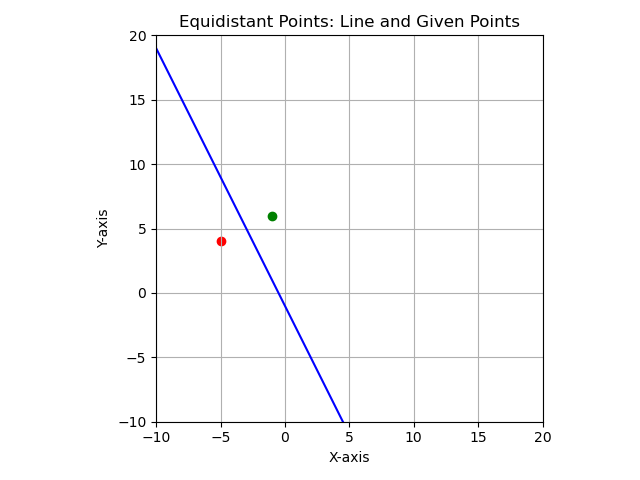
\includegraphics[width=0.6\columnwidth]{figs/equidistant_plot.png}
\caption{Points \(A, B\) and equidistant line \(2x + y = -1\)}
\label{fig:equidistant_plot}
\end{figure}
\end{frame}

\end{document}